\documentclass[a4j,fleqn,10pt]{jarticle}

\usepackage{ipsj}
\usepackage{txfonts}
\usepackage[symbol*,perpage]{footmisc}

\usepackage[dvipdfmx]{graphicx}
\usepackage{url}
\usepackage{subfigure}
\usepackage{latexsym}
\usepackage{multirow}

\newcommand{\birth}[1]{$C(#1)$}
%\newcommand{\distinct}[1]{\mathcal{N}_n^d(#1)}
%\newcommand{\distinctnnn}[1]{\mathcal{N}_3^d(#1)}

%-------------------------------------------jtitle and jauthors information
\begin{document}

\jtitle{逆難読化に向けた適用された難読化手法の特定}
\jcontact{
  京都産業大学
}
\jauthor{匂坂 勇仁 \and 玉田 春昭}

\maketitle

%-------------------------------------------etitle and eauthors information
\footnotetext[0]{\hspace*{-5.2mm}Identifying the applied obfuscation method for de-obfuscation}
\footnotetext[0]{\hspace*{-6.5mm}Hayato Sagisaka \quad Haruaki TAMADA}
\footnotetext[0]{\hspace*{-6.5mm}Kyoto Sangyo University}

%-------------------------------------------document
\section{はじめに}

近年、不正解析など違法行為が増加している。その一対策手法に難読化と呼ば
れる保護手法がある。難読化とは、プログラムの解析を困難にする手法である。
一方、難読化されたプログラムを難読化前のプログラムに戻す逆難読化がある。
逆難読化を行うには、どの難読化が適用されているか特定する必要がある。異
なる方法での逆変換はプログラムを壊すためである.このような逆難読化は保
護を無効にするため、対策が必要である。そこで本稿では保護手法の特定のし
やすさを測定し、保護手法の見つけやすさを計測する.具体的には、難読化さ
れたプログラムを解析し、難読化手法の特徴を探る。我々は、神崎らの不自然
さ評価法\cite{kanzaki14ipsj}を利用した測定を行い,Allatoriという難読化
ツールの特定の可能性を示した\cite{sagisaka15sigss}.本稿では、この研究
をさらに推し進め、より多くの保護手法の特定を試みる.
% 具体的には、5つの難読化手法を適用した9のソフトウェア(jarファイル)の
% 命令を解析し、オペコードの$n$-gramごとの生成確率を得る。またその結果
% が、不明な難読化手法が実際に特定できるかを確かめる。

\section{提案手法}\label{sect:proposedmethod}

\subsection{キーアイデア}\label{sect:keyidea}

図\ref{fig:overview}に提案手法の模式図を示す。図\ref{fig:overview}のよ
うにプログラム$p$を何らかの保護手法$f_1$と$f_2$で保護し,
$p_1=f_1(p)$, $p_2=f_2(p)$を得る。
%
そして、特徴抽出関数$C$を用いて$p$, $p_1$, $p_2$から何らかの特徴
\birth{p}, \birth{p_1}, \birth{p_2}を得る。その後\birth{p}と
\birth{p_1}, \birth{p_2}がどれくらい似ているか、また、\birth{p}と
\birth{q}がどのくらい違うかを評価する。

その後、新たに不明な難読化手法$f_x$で難読化されたプログラム$f_x(p)$を
用意し、提案手法と同様に解析を行う。その結果どの難読化手法が似ているか
を検証する。

\begin{figure}[b]
  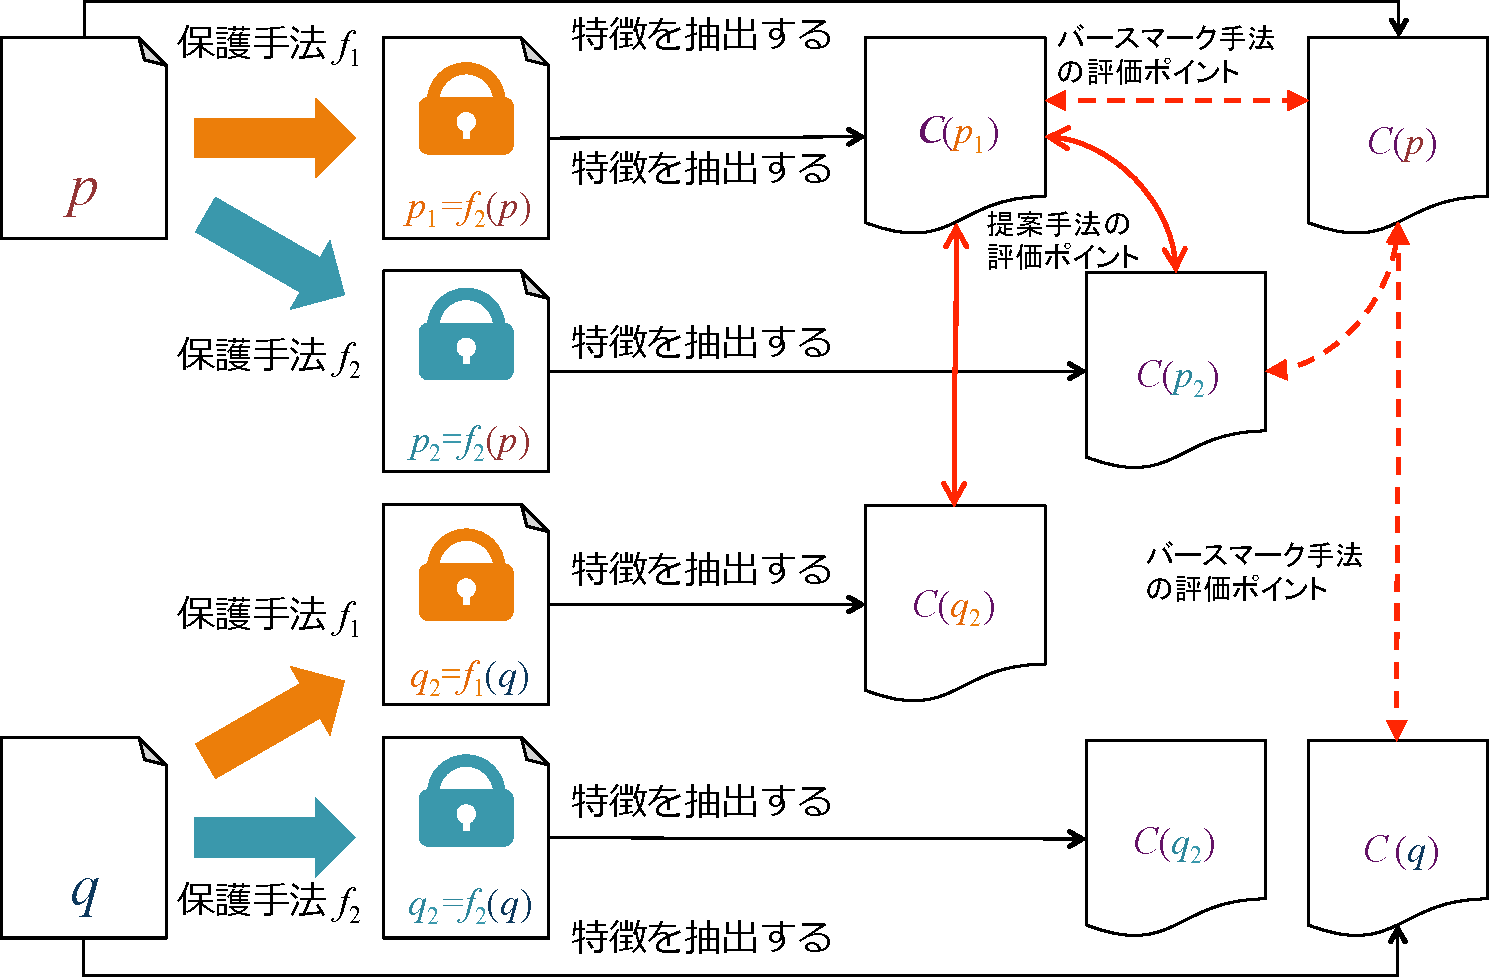
\includegraphics[width=0.48\textwidth]{overview}
  \caption{提案手法の模式図}\label{fig:overview}
\end{figure}

\subsection{特徴抽出法}\label{sect:method}

神崎らが提案した不自然さ評価法に着目する\cite{kanzaki14ipsj}。この手法
は、オペコードの$n$-gramの珍しさを利用するものである。
%
保護手法に現れる命令列の珍しさが保護手法の特徴であると言えるためである。
珍しさを算出するために幾つかの手法が提案されている
\cite{kanzaki14ipsj,gekka14scis}。本稿では,珍しさの算出にパープレキシ
ティを利用する。パープレキシティとは平均分岐数として知られ、言語として
の複雑性を表す指標である。この値が小さいほど、次に来る語が予測しやすい
ことを表す。そのため、値が小さいほど自然であると言える。

一方で、保護手法の中ではコンパイラが出力した本来の命令を重複させる場合
もある。本来の命令は使用頻度の違いはあるものの、珍しいとは言い難い。そ
こで、$n$-gramの頻度にも着目する。
%
このように,プログラムから命令の$n$-gramを抽出し,その珍しさ(パープレ
  キシティ)と頻度を保護手法の特徴とする。

\section{評価実験}\label{sect:experiments}

\subsection{概要}

\begin{table}[t]
  \centering
  \footnotesize{
    \caption{利用したJarファイル一覧}\label{table:jars}
  \begin{tabular}{l|r||l|r||l|r}
    Product & Version & Product & Version & Products & Version \\ \hline
    ASM       & 3.3.1 & FakeHack  & 1.0 &JCalendar & 1.3.3   \\
    Jhstop    & 0.0.1 & Jwhich    & 1.0   & Robocode-setup & 1.6.0.1 
  \end{tabular}
  \caption{利用した難読化ツール}\label{table:tools}
  \begin{tabular}{ll|l}
      Tools & Abbr. & Overview \\ \hline
      Allatori Java Obfuscator & ALL & 商用の難読化ツール \\ \hline
      ProGurad                 & PG & OSSの難読化ツール \\ \hline
      Sandmark                 & & 研究用の難読化ツール \\
      \hspace{0.2cm} Duplication registers & DR & 代入を重複させる.\\
      \hspace{0.2cm} Merge local integers & MLI & 2つのint変数をlongに収める.\\
      \hspace{0.2cm} Irreducibility       & IRR & 制御フローを複雑にする.\\
  \end{tabular}}
\end{table}

本稿では、提案手法により、保護手法ごとの特徴の検出を目的とする。そこで、
Javaを対象とした難読化ツールを用いて、実際にjarファイルを難読化する。
抽出する特徴は、第\ref{sect:method}節で述べたようにオペコードの
$n$-gramを基本とし、そのパープレキシティと頻度を用いて比較を行う。対象
とするJarファイルは表\ref{table:jars}に、難読化ツールは表
\ref{table:tools}に記す。

%%%%追加
その解析結果をもとに、不明な難読化手法の解析を行う。
初めに、未知のプロダクトをケーススタディで扱った
5つの難読化ツール(表\ref{table:tools}をランダムに選択し,難読化する。
そして、どのツールが使われているかを検証する。
次に、既知のプロダクト(表\ref{table:jars})を未知の難読化手法で難読化し、
どのような手法が使われているかを検証する。
未知のプロダクトとしてJUnit 3.7を使用した。
このプロダクトはユニットテストフレムワークである。
また、未知の難読化手法としてSandmarkのSimple Opaque Predicates (SOP) を使用した。
%%%%

\subsection{$n$-gramの分析}

ここでは、$n$-gramの命令列を確認していく。
オリジナルとMLIの頻度順それぞれでソートしたASMを表3に記す。

\begin{table*}[t]
  \centering
  \footnotesize{
    \caption{ASM(5gram)の命令列}\label{table:asm}
  \begin{tabular}{lrrrrrrr}
    命令列 &
    \multicolumn{1}{p{1cm}}{オリジナル} & 
    \multicolumn{1}{p{1cm}}{Allatori} & 
    \multicolumn{1}{p{1cm}}{Duplication} & 
    \multicolumn{1}{p{1cm}}{Irreducibility} & 
    \multicolumn{1}{p{1cm}}{Merge Local Integer} & 
    \multicolumn{1}{p{1cm}}{ProGuard} & 
    \multicolumn{1}{p{1cm}}{PPL} \\ \hline
%    \multicolumn{1}{c}{\rotatebox{90}{オリジナル}} & 
%    \multicolumn{1}{c}{\rotatebox{90}{Allatori}} & 
%    \multicolumn{1}{c}{\rotatebox{90}{Duplication}} & 
%    \multicolumn{1}{c}{\rotatebox{90}{Irreducibity}} & 
%    \multicolumn{1}{c}{\rotatebox{90}{Merge Local Integer}} & 
%    \multicolumn{1}{c}{\rotatebox{90}{ProGuard}} & 
%    \multicolumn{1}{c}{\rotatebox{90}{パープレキシティ}} \\ \hline
    \texttt{<code> <code> <code> <code> aload}      & 219 & 206 & 219 & 219 & 193 & 219 & 61.19 \\
    \texttt{<code> <code> <code> aload getfield}    & 122 &  93 & 122 & 122 & 108 & 122 & 659.44 \\
    \texttt{aload getfield ifnull aload getfield}   & 37  &  22 &  37 &  36 &  37 &  37 & 2478.75 \\
    \texttt{istore iload aload arraylength ifcmpge} & 32  &   1 &  32 &  31 &  19 &  32 & 2305.93 \\
    \texttt{aload ldc invokespecial gotoInsh aload} & 30  &     &  30 &  30 &  30 &  30 & 7249.22 \\
  \end{tabular}
  \begin{tabular}{lrrrrrrr}
    命令列 &
    \multicolumn{1}{p{1cm}}{オリジナル} & 
    \multicolumn{1}{p{1cm}}{Allatori} & 
    \multicolumn{1}{p{1cm}}{Duplication} & 
    \multicolumn{1}{p{1cm}}{Irreducibility} & 
    \multicolumn{1}{p{1cm}}{Merge Local Integer} & 
    \multicolumn{1}{p{1cm}}{ProGuard} & 
    \multicolumn{1}{p{1cm}}{パープレキシティ} \\ \hline
%    \multicolumn{1}{c}{\rotatebox{90}{オリジナル}} & 
%    \multicolumn{1}{c}{\rotatebox{90}{Allatori}} & 
%    \multicolumn{1}{c}{\rotatebox{90}{Duplication}} & 
%    \multicolumn{1}{c}{\rotatebox{90}{Irreducibity}} & 
%    \multicolumn{1}{c}{\rotatebox{90}{Merge Local Integer}} & 
%    \multicolumn{1}{c}{\rotatebox{90}{ProGuard}} & 
%    \multicolumn{1}{c}{\rotatebox{90}{パープレキシティ}} \\ \hline
    \texttt{dup2X2 lxor lconst1 lneg bipush}   &     &     &     &     & 291 &     & 1.13E+06 \\
    \texttt{lload dup2X2 lxor lconst1 lneg}    &     &     &     &     & 291 &     & 536547 \\
    \texttt{aload lload bipush lshr l2i}       &     &     &     &     & 253 &     & 5141.94 \\
    \texttt{<code> <code> <code> <code> aload} & 219 & 206 & 219 & 219 & 193 & 219 & 61.19 \\
    \texttt{bipush lushr land lxor lstore}     &     &     &     &     & 187 &     & 52136.3 \\
  \end{tabular}}
\end{table*}



表3を見ると難読化手法の保護前後で違った命令列が数多くみられる。
また、パープレキシティの値から、珍しい並びであることもわかる。
図2のグラフを見ると保護後には追加の命令が何回も呼び出されている。

\begin{figure}[b]
  \centering
  \begin{minipage}[t]{0.49\textwidth}
  \subfigure[オリジナル]{
    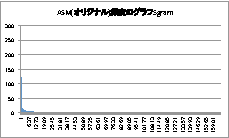
\includegraphics[clip,width=0.47\textwidth]{1}
  }
  \subfigure[Merge Local Integer]{
    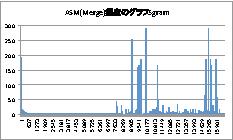
\includegraphics[clip,width=0.47\textwidth]{2}
  }
  \end{minipage}
  \caption{ASM(5gram)頻度のグラフ}\label{fig:graph}
\end{figure}


これらのデータから難読化手法の特徴を表4に示す。

\begin{table}[t]
  \centering
  \footnotesize{
    \caption{ツールごとの特徴}\label{table:caractor}
  \begin{tabular}{l|l}
    ツール              & 特徴 \\ \hline
    Allatori            & オリジナルの命令列をSwap命令で入れ替える \\
    ProGuard            & オリジナルと変化なし \\
    Duplication         & istore命令を2回続けて呼び出す \\
    Merge Local Integer & Dup2X2 lxorと連続した命令がある \\
    Irreducibility      & nop命令がある \\
  \end{tabular}}
\end{table}

\subsection{既知の難読化手法の特定}
ここでは、未知のプロダクトをランダムに難読化し、
どの難読化手法が使われているかを検証する。
解析した結果を頻度順にソートし、表5に記す。
\begin{table}[t]
  \centering
  \footnotesize{
    \caption{junit(5gram)の命令列}\label{table:junit}
  \begin{tabular}{lrr}
    命令列 & 
    \multicolumn{1}{p{1cm}}{不明な難読化手法} & 
    \multicolumn{1}{p{1cm}}{パープレキシティ} \\ \hline
%    \multicolumn{1}{c}{\rotatebox{90}{オリジナル}} & 
%    \multicolumn{1}{c}{\rotatebox{90}{Allatori}} & 
%    \multicolumn{1}{c}{\rotatebox{90}{Duplication}} & 
%    \multicolumn{1}{c}{\rotatebox{90}{Irreducibity}} & 
%    \multicolumn{1}{c}{\rotatebox{90}{Merge Local Integer}} & 
%    \multicolumn{1}{c}{\rotatebox{90}{ProGuard}} & 
%    \multicolumn{1}{c}{\rotatebox{90}{パープレキシティ}} \\ \hline
    \texttt{dup2X2 lxor lconst1 lneg bipush}     & 16 & 1.13E+06 \\
    \texttt{lload dup2X2 lxor lconst1 lneg}      & 16 & 536547 \\
    \texttt{bipush lushr land lxor lstore}       &  9 & 52136.3 \\
    \texttt{lconst1 leng bipush lushr land}      &  9 & 96291.9 \\
    \texttt{lneg bipush lushr land lxor}         &  9 & 136813 \\
  \end{tabular}}
\end{table}

表5を見るとオリジナルから追加されている命令列がある。
その命令列を特徴とし、5つのツールの特徴と比較する。
追加命令列には、dup2X2 lxorといったパープレキシティの値が高い命令列がある。
その特徴と第3.2節で得た表4を比較する。その結果、Merge手法の特徴が当てはまった。

\subsection{未知の難読化手法の特定}
ここでは、既知のプロダクトを未知の難読化手法で難読化を行い、
どの難読化手法が使われているかを検証する。
解析した結果を頻度順にソートし、表6に記す。

\begin{table}[t]
  \centering
  \footnotesize{
    \caption{jhstop(5gram)の命令列}\label{table:jhstop}
  \begin{tabular}{lrr}
    命令列 &
    \multicolumn{1}{p{1cm}}{未知の難読化手法} & 
    \multicolumn{1}{p{1cm}}{パープレキシティ} \\ \hline
%    \multicolumn{1}{c}{\rotatebox{90}{オリジナル}} & 
%    \multicolumn{1}{c}{\rotatebox{90}{Allatori}} & 
%    \multicolumn{1}{c}{\rotatebox{90}{Duplication}} & 
%    \multicolumn{1}{c}{\rotatebox{90}{Irreducibity}} & 
%    \multicolumn{1}{c}{\rotatebox{90}{Merge Local Integer}} & 
%    \multicolumn{1}{c}{\rotatebox{90}{ProGuard}} & 
%    \multicolumn{1}{c}{\rotatebox{90}{パープレキシティ}} \\ \hline
    \texttt{irem iconst0 ifIcmpne aload getfield}     & 15 & 15394.6 \\
    \texttt{dup dup dup imul imul}                    & 14 & 4.24E+06 \\
    \texttt{dup dup imul imul isub}                   & 14 & 874418 \\
    \texttt{dup imul imul isub iconst3}               & 14 & 348582 \\
    \texttt{iload dup dup dup imul}                   & 14 & 1.01E+07 \\
    \end{tabular}}
\end{table}

表6を見ると、dup ,imul命令を複数呼び出している。
その特徴と第3.2節で得た表4を比較する。
しかし、難読化手法の特徴と似たものがなかった。
 次に、未知の難読化手法を別のプロダクトで難読化し、同様に比較を行った。
 その結果、未知の難読化手法の判別が可能となった。
 
 \section{まとめ}

 本稿では不自然さ評価に着目して、適用された保護手法の特定に取り組んだ。
実際のプログラムに、5種類の保護手法を適用し、$n$-gramの命令列を頻度順に確認した。
その結果をもとに不明な難読化の解析を行った。
今回の結果を参考に逆難読化の研究に取り組むことが今後の課題である。


%-------------------------------------------references
\bibliographystyle{junsrt}
\bibliography{sagisaka}

\end{document}
